\section{Melting in a retained aluminium backing}\label{sec:almelt}
The original aluminium cases use constant specific heat. The alternative
stores the heat of fusion and allows the backing to become liquid while
retaining its initial mass, shape, radial conductivity of 167 W/(m K) and
density of 2700 kg/m$^3$. Gas loading, liner chemistry and dimensions match the
nominal cases in Table~1. The extra heat absorbed by the casing delays liner
exhaustion by 3.7 s in the sustainer and 5.2 s in the booster.

\begin{table}[H]\centering\begin{tabular}{lrrrrr}\toprule
 & Property & First & All cells & Liner & Liner at full\\
Case & flag [s] & melt [s] & liquid [s] & gone [s] & melt [mm]\\\midrule
Sustainer & 50.7 & 84.1 & 99.1 & 110.5 & 0.43 \\
Booster & 84.4 & 124.4 & 139.4 & 147.6 & 0.23 \\
\bottomrule\end{tabular}\end{table}
\begin{figure}[H]\centering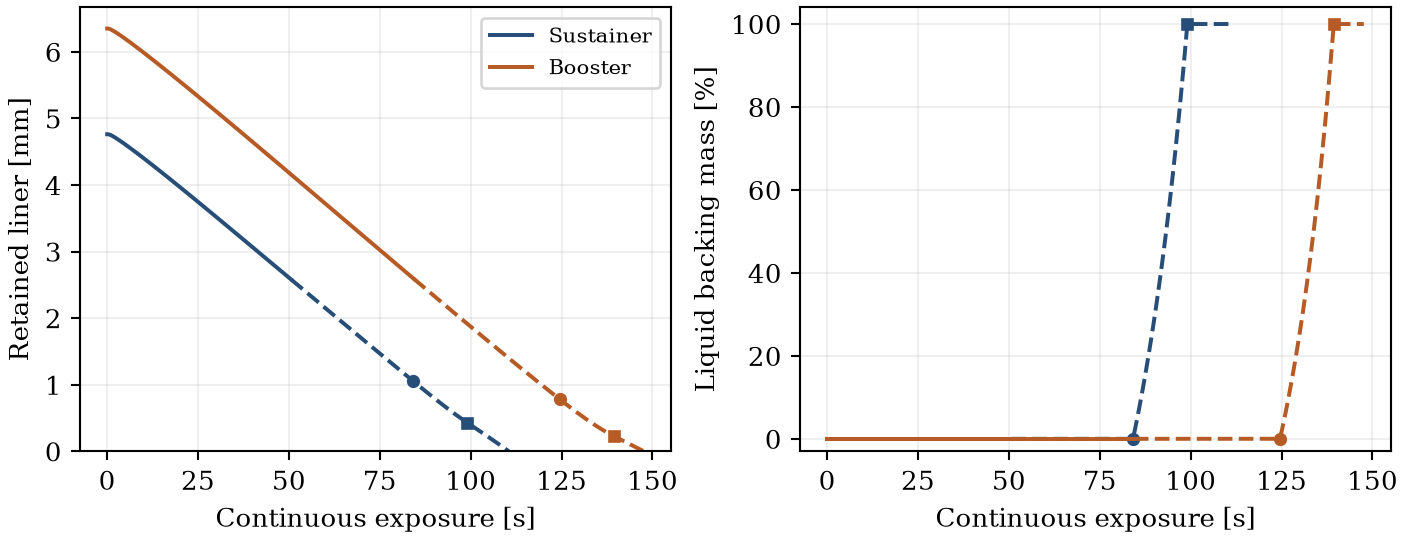
\includegraphics[width=\textwidth]{../analysis/al_backing_phase.png}
\caption{Solid curves end at the inherited 300 $^\circ$C property flag. Dashes
continue with the retained pure-Al surrogate. Circles mark the first cell with
liquid and squares mark the first instant when all casing cells are liquid.}\end{figure}
At complete modelled melting the liner still covers the case in both geometries.
Following the liner further assumes the liquid stays in place. Pressure
containment, flow of molten metal, alloy solidus and local wall defects need
separate evidence.

The caloric law uses the crystal and liquid rows on the same
\href{https://janaf.nist.gov/tables/Al-001.html}{NIST-JANAF enthalpy reference}.
At 933.45 K the 10.711 kJ/mol jump corresponds to 397.0 kJ/kg. The solver joins
the two sensible branches across a narrow numerical melting interval, then
recovers liquid fraction from the sharp equilibrium enthalpy. Ten integrations
separate mesh, time-step and interval-width changes. The reported runs use
640/160 cells, a 0.02 s step ceiling and a 0.5 K interval. Across the eight
single-parameter comparisons the greatest liner-event shift was 0.007 s.
All eight satisfy the thickness and final-interval overlap checks. An externally
heated char/Al coupon agrees with an independent sharp-transition enthalpy ODE
to 0.25 K at the finest setting.

\clearpage\section{Resin reaction on the CF temperature histories}\label{sec:cfdiag}
A separate calculation applies the two competing T700/M21 reactions measured
under nitrogen to the liner-side and outside temperatures of the published
CF cases. The heat histories are prescribed. Heat absorption, gas transport
and the changing composite conductivity would have to feed back into the wall
to revise a CF liner-exhaustion time.

Let $u=1-a_1-a_2$ denote the fraction of the shared reactant still available.
With $T$ in kelvin and $k_j=A_j\exp[-E_j/(RT)]$ in s$^{-1}$, the rates are
\[
 \dot a_1=k_1 u^{1.1125},\qquad \dot a_2=k_2 u^{2.0825}(1+K_{\rm cat} a_2).
\]
The frequency factors are 7.2193 and $5.3309\times10^8$ s$^{-1}$, and the
activation energies are 58.7107 and 146.674 kJ/mol. The table uses
$K_{\rm cat}=7.4886$ from Table 5 of the experimental paper. The model equations
and competitive mass-loss weights are given in its companion paper.
\href{https://doi.org/10.3390/ma10050494}{Tranchard et al., Part I};
\href{https://doi.org/10.3390/ma10050470}{Part II}.

\begin{table}[H]\centering\begin{tabular}{llrrrr}\toprule
 & & \multicolumn{3}{c}{Time to reactant conversion [s]} & At 50\%\\
\cmidrule(lr){3-5}Case & Casing location & 10\% & 50\% & 90\% & [$^\circ$C]\\\midrule
Sustainer & Liner side & 52.4 & 56.6 & 61.4 & 522 \\
Sustainer & Outside & 71.2 & 75.7 & 80.7 & 520 \\
Booster & Liner side & 80.5 & 85.9 & 91.8 & 514 \\
Booster & Outside & 117.5 & 123.2 & 129.8 & 511 \\
\bottomrule\end{tabular}\end{table}

Here 50\% means half of the common reactive pool has advanced by either
pathway. Reconstructing mass with the paper's density change and pathway
weights gives about 12.3\% loss of the initial composite mass at that point.
The printed $\log_{10} K_{\rm cat}=-0.8744$ in Part I, Table 3 implies
a smaller coefficient. Using that interpretation delays the four 50\% times
by 3.0--4.1 s. The calculations stop at 99.9\% common conversion, 1000
$^\circ$C, or the end of the supplied temperature history, whichever occurs first.

The local rates of temperature rise at 50\% conversion are 492--697
$^\circ$C/min, above the reported nitrogen tests at 5--100 $^\circ$C/min.
The Iris casing resin and layup are unspecified. These times identify when a
reacting backing can affect the heat balance. The following section couples heat storage, radial
conductivity, decomposition energy and escaping gas to both motor geometries.
\clearpage
